\documentclass[10pt,a4paper]{article}
\renewcommand{\baselinestretch}{1}
\usepackage{amssymb,amsmath}            
\usepackage{graphicx}                   
\usepackage{indentfirst}
\usepackage{microtype}
\usepackage{moreverb}
\usepackage{multicol}
\usepackage{hyperref}
\usepackage[utf8]{inputenc}
\usepackage[margin=1.2in]{geometry}

\title{Introduction to Vision and Robotics - Coursework 2 Report}           
\author{Victor Dumitrescu (s1107546), Ignotas Šulženko (s1137931)}                      
\date{27th March 2014} 

\begin{document}
\maketitle


\section{Introduction}\label{introduction}

In this assignment we had to make a Khepera robot navigate by following
a wall and keeping the distance to it constant. The robot is also
supposed to circumvent any obstacles that it might encounter along the
way. For this task we used the Webots simulator and implemented a PI
controller that allows the robot to smoothly follow the wall together
with an odometry system that lets the robot stop when it comes back to
the origin.

\section{Methods}\label{methods}

\subsection{Basic code structure}\label{basic-code-structure}

This is the basic outline of the control flow (in pseudocode):

\begin{verbatim}
while the robot is not stuck and has not finished the lap:
    get the sensor values
    while the robot does not sense anything in front or to its right:
        move forward
    if robot has not reached its starting point:
        if there is an obstacle in front:
            set the robot speeds so that it turns left on the spot
        else calculate PI adjustments to follow the wall:
            calculate errors for the relevant sensors' values
            calculate the left and right motor speeds using P
            calculate the left and right motor speeds using I
            set the robot speeds by combining P and I results
        update the odometry values
        check if we have finished the lap
\end{verbatim}

Our method prioritizes obstacle avoidance over wall tracking in order to
avoid getting stuck in corners or touching the walls.

\subsection{The controller}\label{the-controller}

We decided to use a PI controller for maintaining a constant distance to
the wall as it seemed to offer an optimal solution based on control
theory. In the interest of simplicity, we made the decision to always
follow the wall on the robot's right, but we have implemented the
controller so that it is easy to switch sides or choose between them.

The idea behind the controller is to set an ideal value for each of the
robot's IR sensors, calculate the error at each point and compute
proportional (P) and integral (I) adjustments for each of them. The
adjustments for each motor are then added to their base speed in order
to influence the robot's trajectory. In practice, we have decided to
only use the input from 2 of the sensors (the rightmost and top-right
one) for the PI controller.

We started with implementing the P component, which worked reasonably
well on its own, after calibrating with the correct gains. In order to
enable us to have larger speeds for our robots while also avoiding
overshooting the trajectory we also implemented the integral component.
With proper calibration, we found that our robot is able to maintain a
fairly constant distance from the wall it is following. More detailed
experimental results follow in the next section.

In the code, each component of the controller is implemented as a
separate function in \texttt{kheperam/controllers/task1/}:
\texttt{p\_component.m} and \texttt{i\_component.m}.

\subsection{Obstacle avoidance}\label{obstacle-avoidance}

Although we had code that could make the robot follow the wall, we had
to use some different approach to be able to escape from corners and
avoid obstacles. At first, we tried running our robot with using just
the front and the rightmost sensors (sensors 2, 3 and 5) and checked if
there is an obstacle in front of the robot and in case there is
something, we would turn on the spot. Unfortunately, after some tests we
discovered that this simple approach does not always work - the robot
fails to avoid corners of narrow blocks. It was tending to cur corners
because it would no longer sense an obstacle in front and the distance
as measured by the rightmost sensor would not be enough to determine
whether we're following a wall or circumventing an obstacle.

\begin{figure}[htbp]
\centering
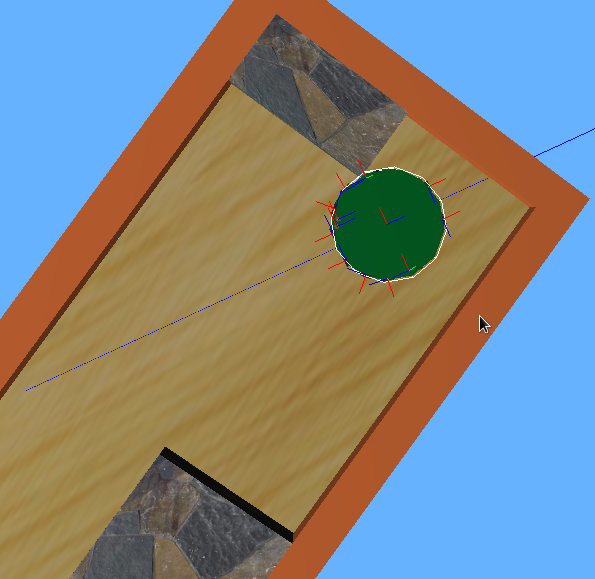
\includegraphics[width=10cm]{images/obstacle_avoidance_fail.png}
\caption{Robot fails to avoid a corner of a narrow block}
\end{figure}

In order to make the robot avoid every kind of obstacles we redesigned
our algorithm to also use the sensor on the right diagonal (sensor 4)
when checking for an obstacle. After a little a bit of experimentation
with distance threshold values for the obstacle avoidance, we found a
configuration which seems to solve all of our problems. As described in
the Results section, however, making our robot avoid all obstacles meant
incurring a small penalty on the time that it takes to stabilize the
path after the robot passes an obstacle or takes a corner. This can
happen because checking whether the robot is facing an obstacle will
sometimes return a false positive and will engage briefly in obstacle
avoidance even though the robot is just following the wall. However, the
trajectory eventually stabilizes.

\subsection{Odometry}\label{odometry}

Odometry is necessary to make the robot stop after completing a lap in
the maze. Therefore, we adopted the solution suggested in the Practical
5 of Khepera robot control on Week 6 which uses the speed of the left
and right wheels in order to determine the current position and the
angle of the robot:

\begin{figure}[htbp]
\centering
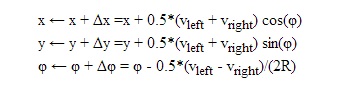
\includegraphics{images/Odometry_formulae.png}
\caption{Odometry formulae}
\end{figure}

After implementing this, we discovered that taking the \textbf{speeds}
of the motors does not produce accurate results because they have slip
noise associated with them. Therefore we started registering the actual
wheel \textbf{rotation counts} to update the inner robot coordinate and
angle representation, which works way more precisely. We stop the robot
whenever the Euclidean distance from the origin point to the current
robot location is within 10 millimetres, which is pretty accurate for
our purposes.

\section{Results}\label{results}

\subsection{Robot control: following the
wall}\label{robot-control-following-the-wall}

Generally, the robot manages to follow a path close to the wall at a
relatively constant distance. The following graph shows the reading of
the rightmost proximity sensor while initially approaching a wall at an
angle of approximately 45 degrees. The time step between each reading is
128ms. This shows that the PI controller is able to stabilize the
robot's trajectory within 3.2s of reaching the goal distance for the
first time. The base speed of the robot is 2.4cm/s.
\begin{center}
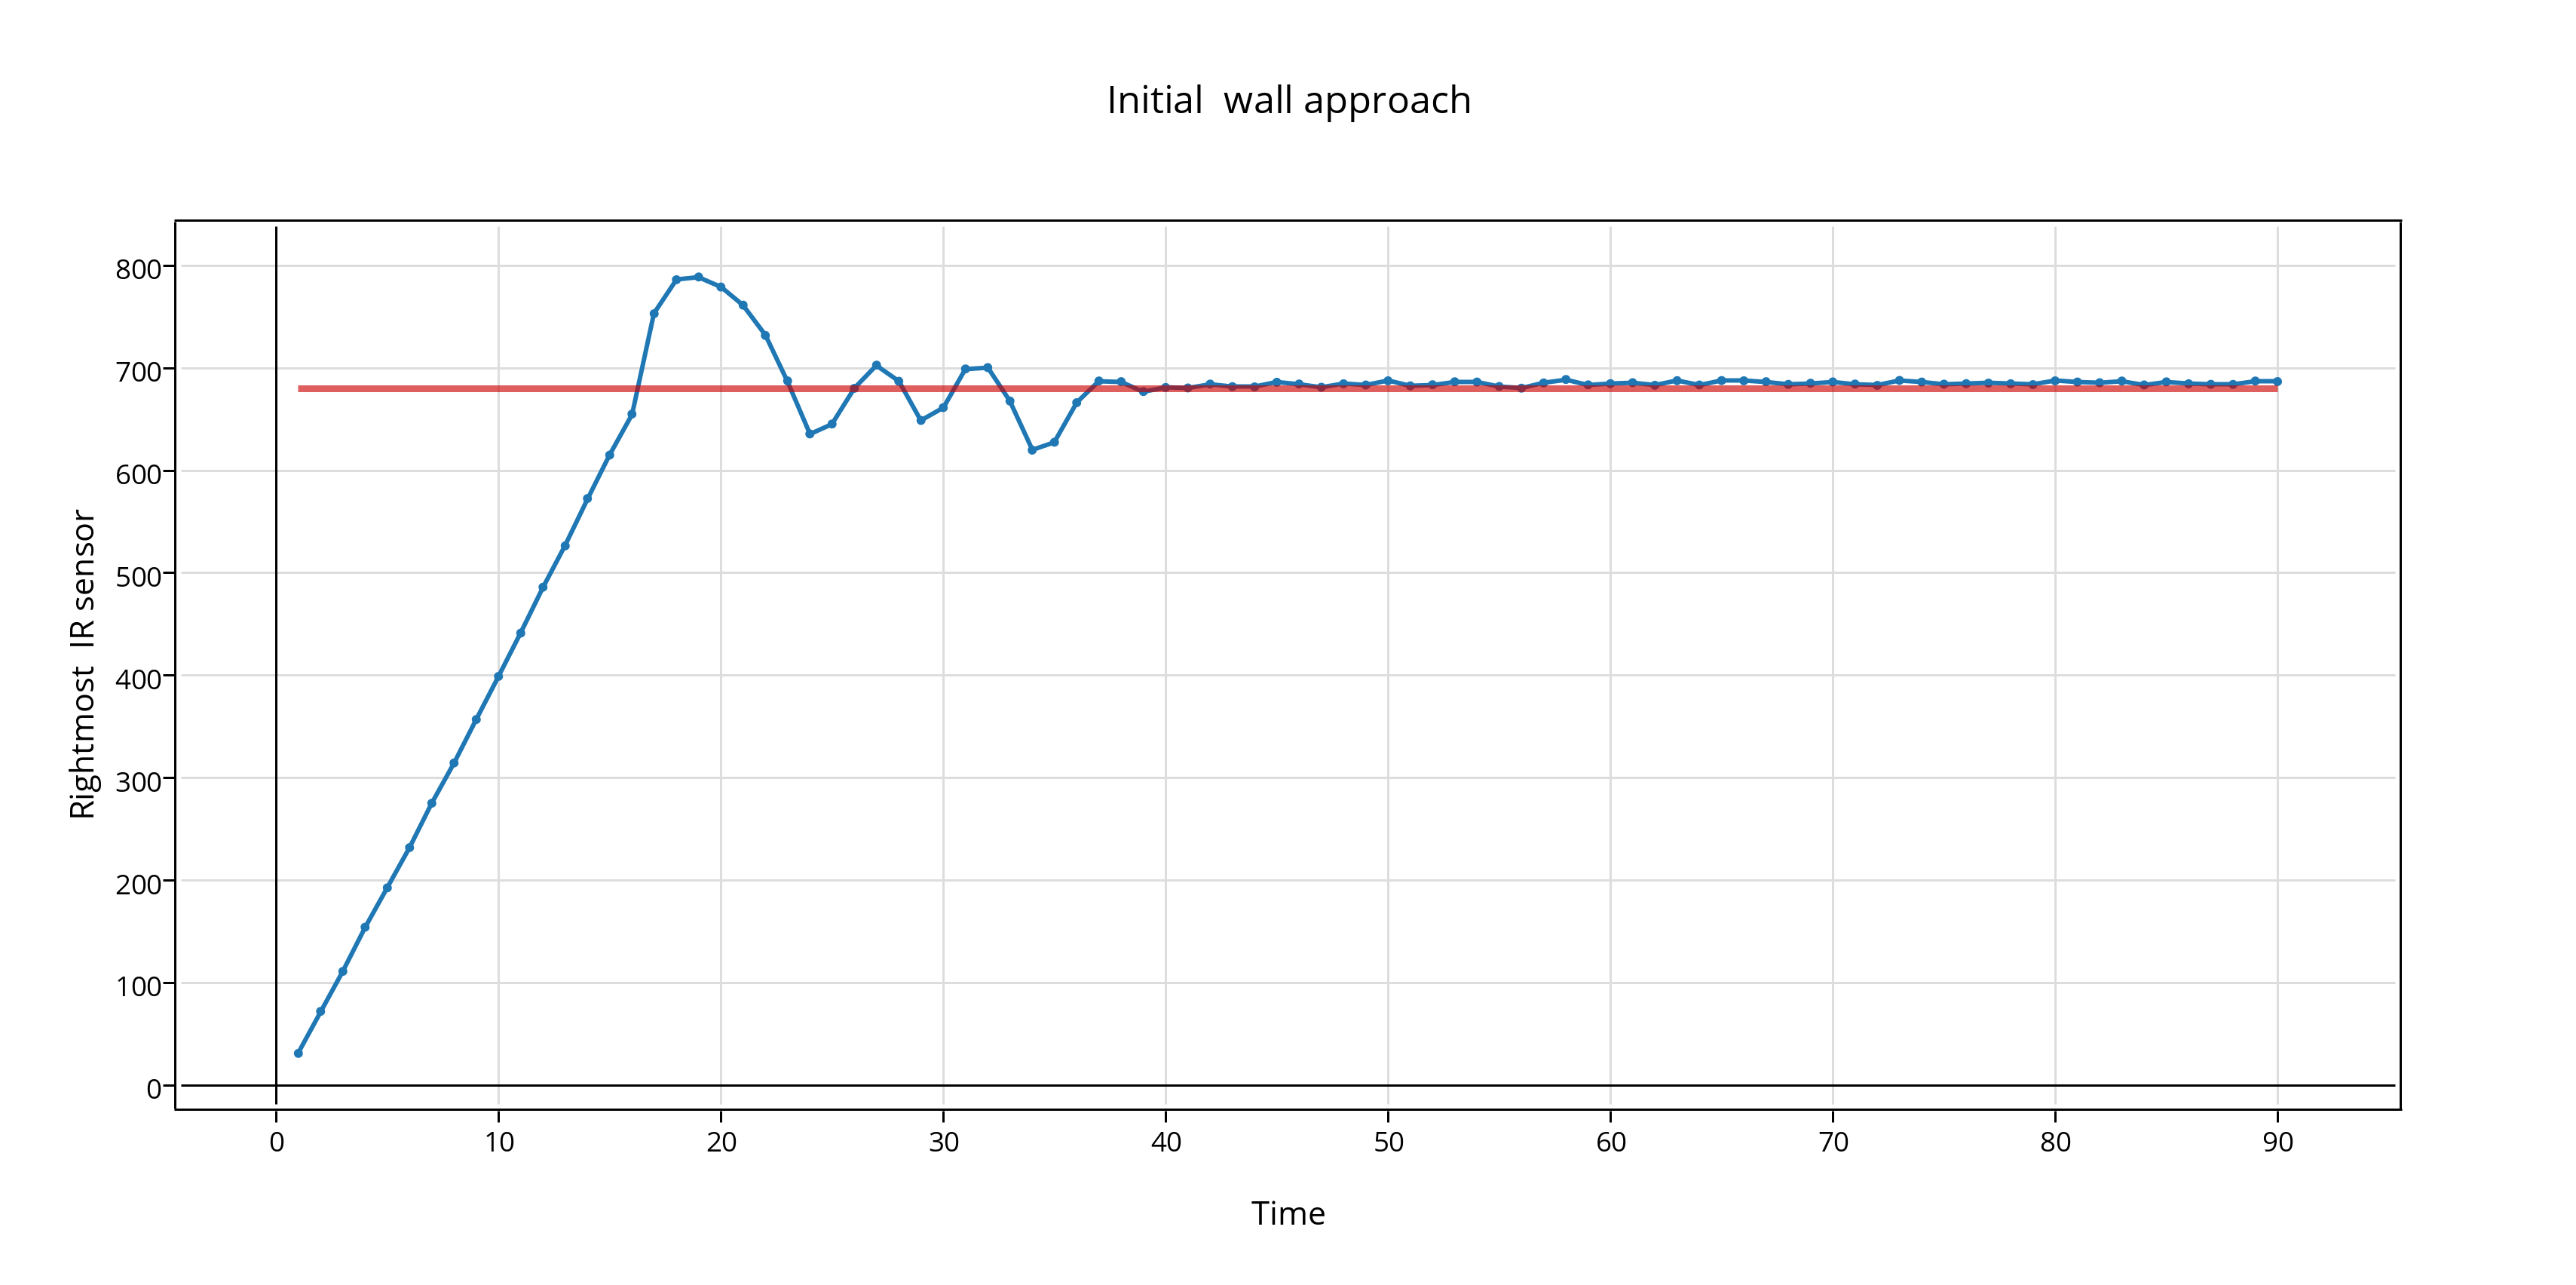
\includegraphics[width=15cm]{images/initial_wall_approach.png}
\end{center}

\begin{samepage}
In our testing we have found that it usually takes less time to recover
from corners or obstacles. The graph below shows both the rightmost and
the top-right sensor readings while taking a corner:

\begin{center}
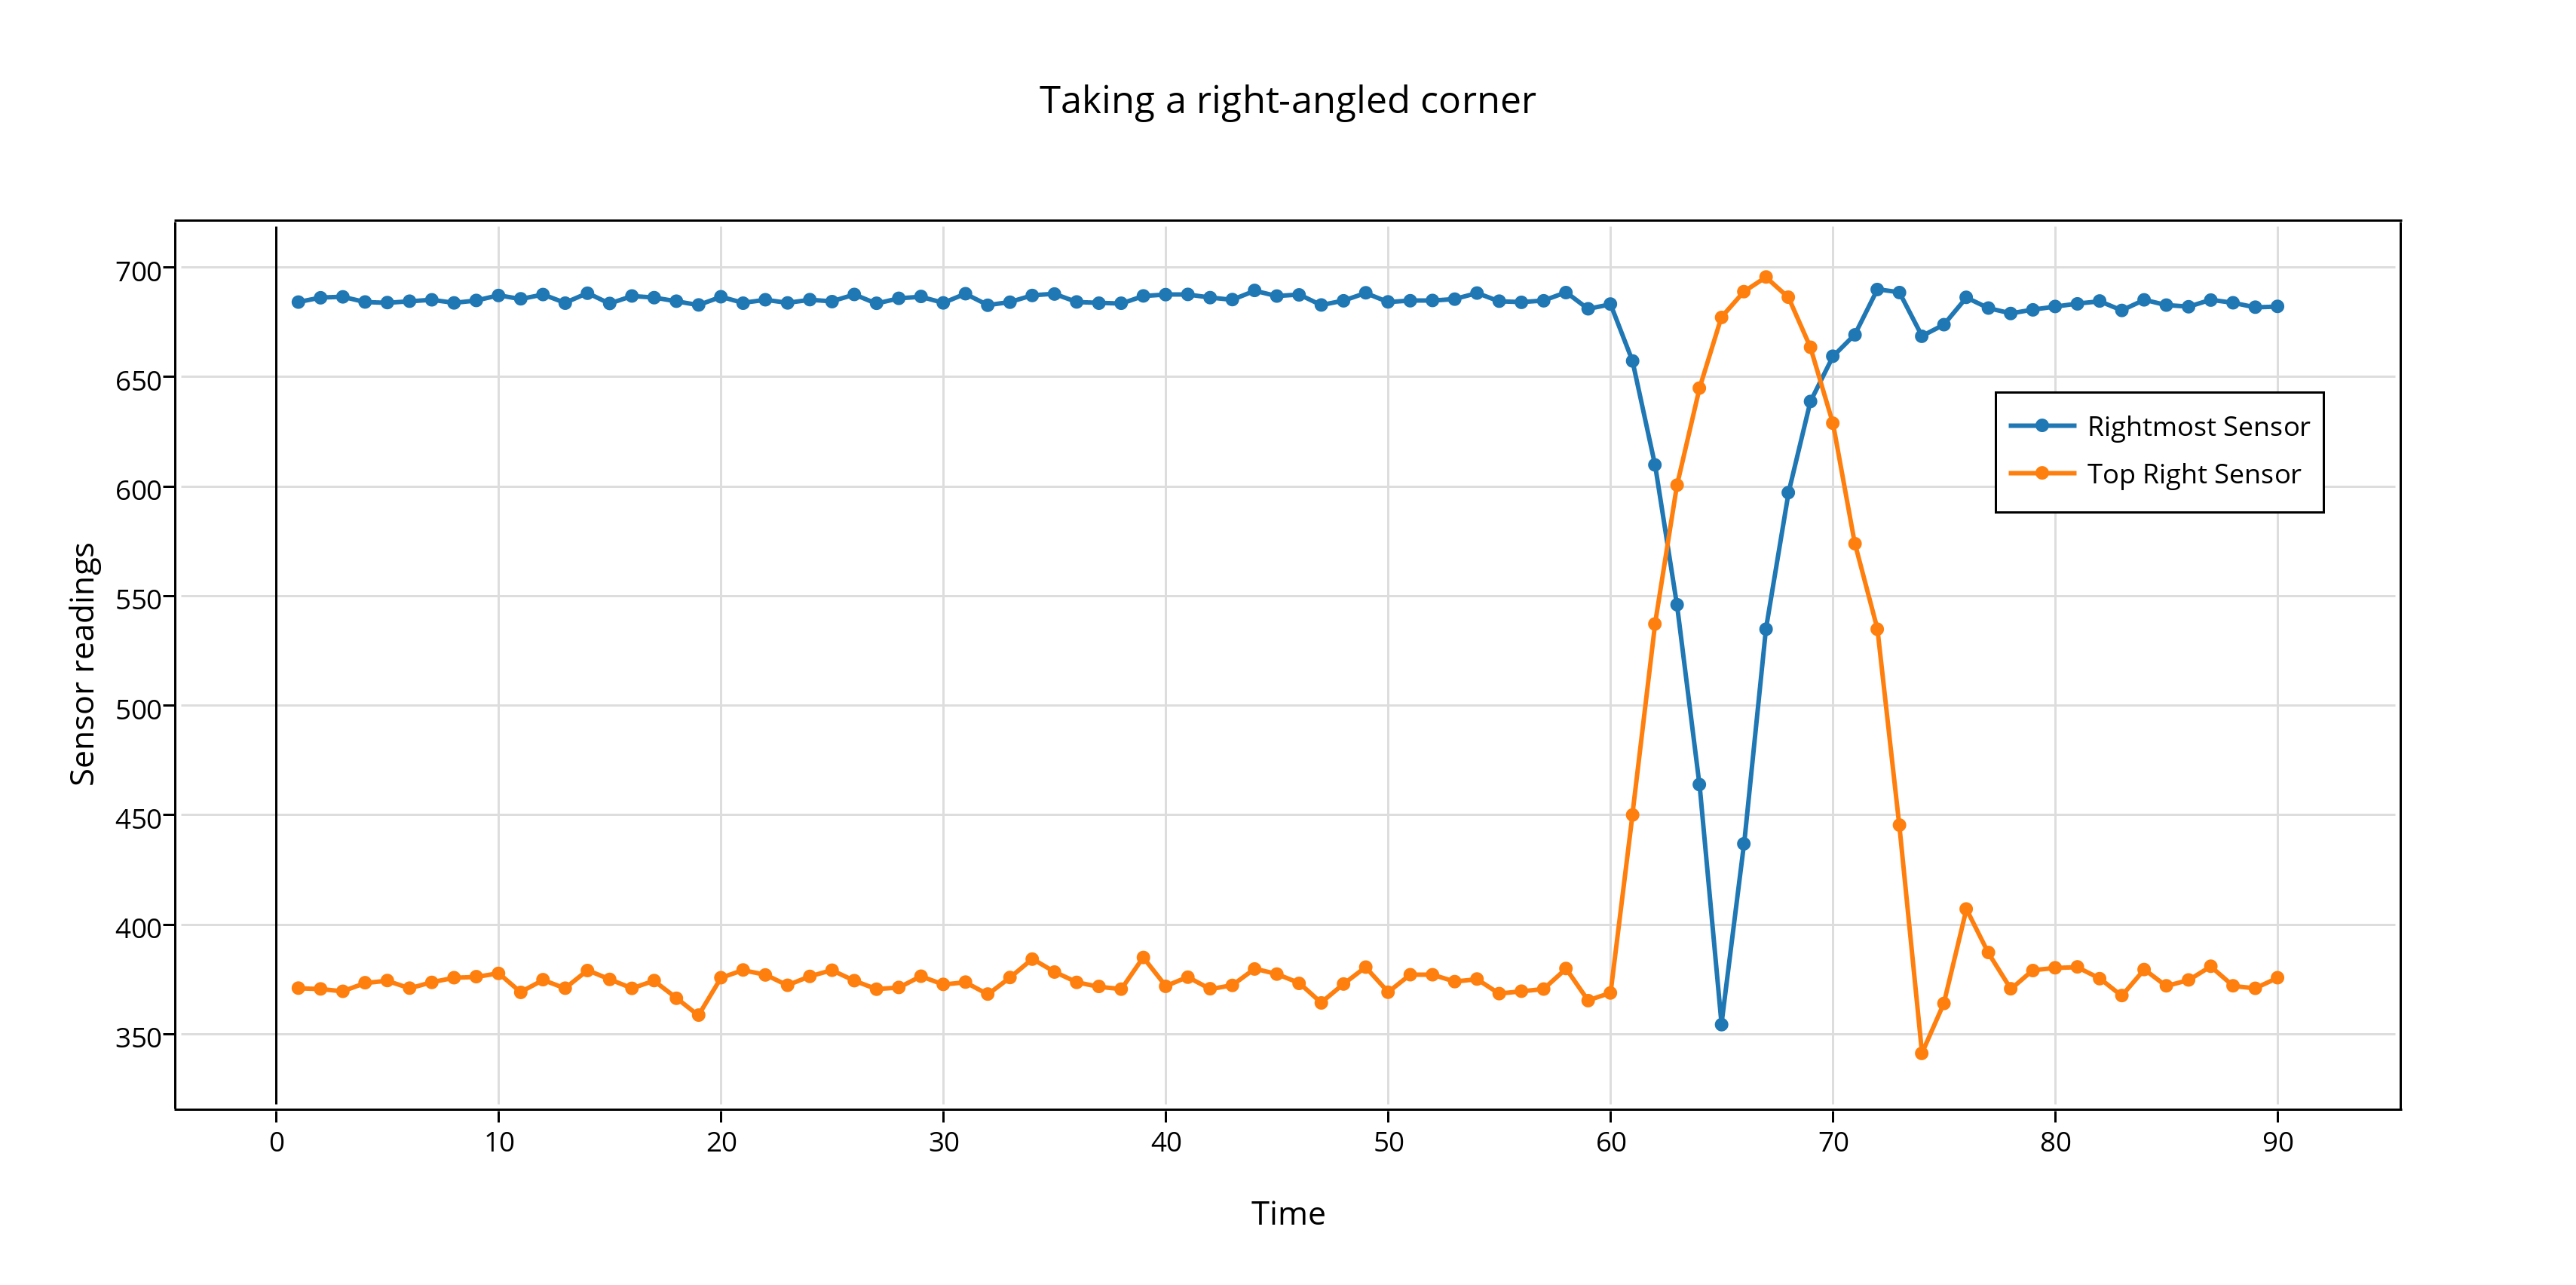
\includegraphics[width=15cm]{images/taking_a_right-angled_corner.png} 
\end{center}
\end{samepage}

In this case,
the trajectory is largely recovered in less than 2s. This is
representative of all the corner cases in our trials. This plot of the
robot's position overlayed with an empty rectangular road shows that
following the wall and taking corners is done smoothly in the absence of
obstacles. 

\begin{center}
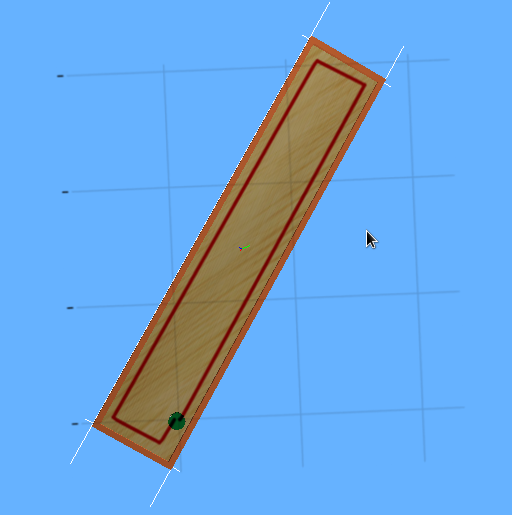
\includegraphics[width=7cm]{images/empty_world_overlay.png}
\end{center}

\subsection{Robot control: navigating around
obstacles}\label{robot-control-navigating-around-obstacles}

Our final version of the robot manages to avoid rectangular obstacles of
different shapes and sizes. A lot of calibration and changes of the
rotation logic were necessary in order to avoid getting the robot stuck
in the sharp edges of these obstacles, as illustrated below. We were
faced with a trade-off between sometimes getting stuck in these corners
and speedy recovery of a straight trajectory after an obstacle is
passed. We chose to optimise for the former.

\begin{center}
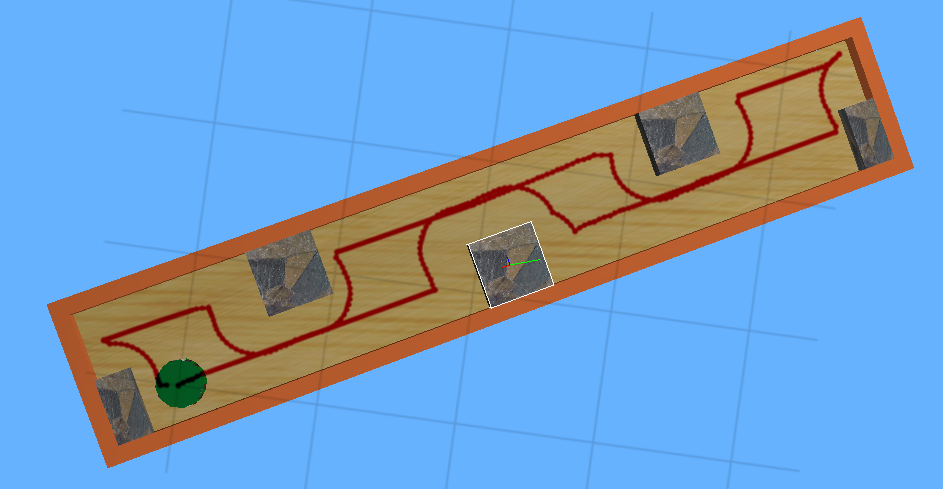
\includegraphics[width=12cm]{images/world1_overlay.png}
\end{center}

This assures that our robot has the highest chance of navigating the whole path, even though speed
might slightly suffer in some cases where the trajectory oscillates for
a longer interval. 

\begin{center}
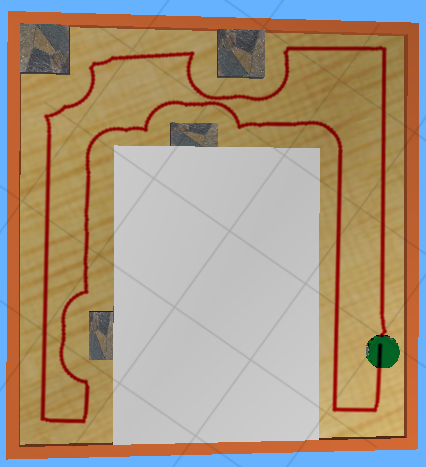
\includegraphics[width=7cm]{images/world2_overlay.png}
\end{center}

\emph{\textbf{Note:} These images are not 100\% accurate as they were
hand-aligned with the plot of the trajectories. They are intended to
demonstrate how the obstacles are navigated, but the don't provide an
accurate estimation of the distance between the robot and the different
elements of the world.}

\begin{multicols}{2}
\section{Discussion}\label{discussion}

We believe our results above show that we have been quite successful in
making the robot autonomously navigate by following a wall, avoid
different kinds of obstacles and stop precisely at the origin point.
However, we realise that there are some limitations to our
implementation and there are improvements that we could make.

First of all, based on the assignment description, we assumed
throughout that all obstacles are rectangular-shaped objects. Our
obstacle avoidance algorithms have been tailored to avoid rectangular
objects and might therefore fail when trying to avoid V-shaped objects
or objects that have cavities that are too narrow for the robot. In order
to solve this problem, we would have to implement a more robust obstacle
avoidance algorithm that possibly uses \textbf{all 8} of the sensor
values and not just the 3 sensor values as it is doing currently.

Finally, we could try to make the robot move faster and increase the
fluidity of its movements. For that we would need to implement the
Derivative controller and use it in addition with the Proportional and
Integral controllers. Although with the current speed of the robot, our
controller does not have significant difficulties in achieving and
maintaining the desired distance from the wall, an increase in speed
would make the movement more jerky and less accurate, so a Derivative
controller would become necessary.

\section{Work distribution}\label{work-distribution}

\paragraph{} We have both made similar contributions to the assignment and thus the
split should be 50:50. 
\paragraph{} \emph{Victor -} I have implemented the PI
controller and developed an initial structure of our code based on the
one provided in the assignment files. I have implemented an initial
obstacle avoidance logic and spent some time trying to find the optimal
gains and parameters. 
\paragraph{} \emph{Ignotas -} I have implemented the odometry
and made the robot stop when it reaches the origin after completing a
lap. Also, I have experimented with the obstacle avoidance logic and
contributed some changes to it, refactored parts of the code for
clarity. 
\paragraph{} \emph{Both -} We finalised the structure of our code together
and consulted in order to improve each other's approaches and
implementation. We tested the robot both individually and together. We
worked together on writing this report.

\end{multicols}

\end{document}
